\documentclass[a4paper]{article}

\usepackage[english]{babel}
\usepackage[utf8]{inputenc}
\usepackage[round]{natbib}
\usepackage{amsmath}
\usepackage{graphicx}
\usepackage{url,hyperref,lineno,microtype}
\usepackage[onehalfspacing]{setspace}
\def\keyFont{\fontsize{8}{11}\helveticabold }
\linenumbers

\title{Characterizing rice pest injury co-occurrence patterns at different irrigated lowland rice growing areas by network analysis}

\author{Sith Jaisong}

\date{\today}

\begin{document}
\maketitle

\begin{abstract}

Knowledge of the network structure of rice pest injury co-occurrence patterns helps to understand the formation and characteristics of injury profiles at different rice growing areas in South and Southeast Asia. Therefore, survey data of 420 rice fields over three years across 5 countries, India, Indonesia, Philippines, Thailand, and Vietnam were investigated. The aim of the study was to use network analysis to characterize the patterns of pest injury co-occurrence in specific locations and to determine the key pests using the properties of the network. The results of the weighted co-occurrence networks indicated that ???. Therefore, network analysis provides insights into the pattern of co-occurrence  which could be of particular interest for the identification of key factors with regard to different rice growing locations. .......

\end{abstract}

\section*{Introduction}
In nature, growing plants can frequently be infected at the same time by more than one species of pests and pathogens. These plant enemies caused injuries, which possibly affect yield productions when they are severe. Crop health is highlighted and implemented to manage a combination of injuries, so-called injury profiles. The co-occurrence patterns of injury are beginning to provide important insight into the injury profiles, which possibly present co-occurring or anti-co-occurring relationships between injury-injury. Uncovering these patterns might have important to implications in plant disease epidemiology and management. However, there are only a few reports of injury–injury interactions in crop systems and the mechanisms of interactions are currently unknown and this could be a difficult task since complex patterns of injury profiles are related to environmental conditions, cultural practices, and geography \citep{willocquet2004research}.

To address this issue, we use in-field surveys as a useful tool to develop ground-truth databases that allow one identify actual constraints due to pests in an agricultural productions system. These sorts of databases provide an overview of the complex relationships between the crop, its management, pest injuries, yields. Several previous studies \citep{Savary:2000char, savary2000quanti, savary2005multiple, dong2010characterization, Reddy:2011hl} involved surveys that have been used to identify relationships in an individual production situation (a set of factors including cultural practices, weather condition, socioeconomics, \textit{etc} that determine agricultural production ) and the injury profiles using nonparametric multivariate analysis such as cluster analysis, correspondence analysis, multiple correspondence analysis. Performing correspondence analysis \citep{savary1997new}, they characterized the relationships between categorized levels of variables: actual yield, production situations, and injuries profiles. For example, stem rot and sheath blight are frequently found together with high (mineral) fertilizer inputs, low pesticide use, and good water management in transplanted rice crops and overall, their results led to the conclusions that observed injuries profiles were strongly associated with production situations and the level of actual yields. 

We applied the technique from ecological study the co-occurrence analysis and network theory to reveal the patterns of co-occurrence of injury profiles. While existing statistic approach for analysis the survey data e.g. cluster analysis, correspondence analysis, multiple correspondence analysis, the methods were present in this papers has the advantages of ........

Network theory is the study of relationships between entities (`nodes') and connections between these entities (`edges'). Network theory has previously been used effectively to describe social and biological datasets, and it has been shown to be a useful tool for ???. Here, we consider pest injuries as nodes and create an edge between any two injuries if they are co-existing. We give an edge greater weight if the two injuries have strong co-occurrence at either end.  The relationships will be more complex when the number of their components increased. A way to systemically model and intuitively interpret such relationships is the depiction as a graph or network. This approach has been widely used and proven very useful in biological studies \citep{Lefebvre:2011fo}. Networks typically consist of nodes, usually representing components, while links between the nodes depict their interactions \citep{PROULX:2005hx}. A correlation network is a type of network in which two nodes are connected if their respective correlation lies above a certain threshold. The construction of this network is obtained from pairwise correlation methods \citep{Toubiana:2013cv}. By using appropriate correlation measure, correlation networks can capture biologically meaningful relationships, and discover valuable information in crop health surveys.

The aim of this study was to analyze how the structure of correlation network of pest injury co-occurrence are different over 5 locations under investigation (West Java, Indonesia, ??, India, Laguna, Philippines, Central plain, Thailand, and Makhong river delta, Vietnam). By quantifying the important aspects of the position of the specific pest injury, information based on network analysis could help to understand the formation and characteristics of co-occurrence patterns. Furthermore, key factors for could be identified with this additional information.

%===================================I maybe change the material and methods ================================
\section*{Materials and Methods}

\subsection*{Study sites, sampling and data collection}
We conducted the surveys located in the South and South East Asia, Kerala, India(Lat , Long), Indonesia (Lat , Long), Philippines (Lat , Long), Central Plain, Thailand (Lat , Long), and Mekong Delta Vietnam (Lat , Long). Theses are the important rice growing areas, where use irrigated lowland rice ecosystem.  intensive condition, which grow twice per year. We sampled in , under same standardized protocol described in the IRRI publication, ``A survey portfolio to characterize yield-reducing factors in rice'', was used for data collection \citep{Savarysurvey2009}.

\begin{figure}[h!]
\begin{center}
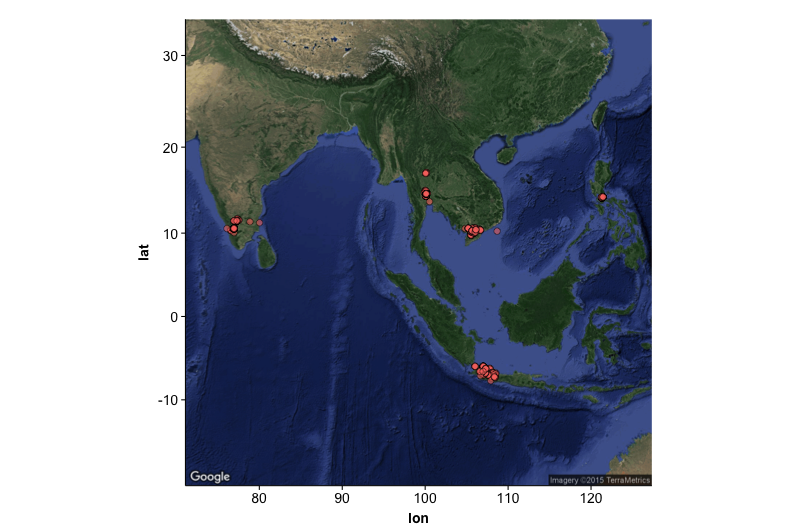
\includegraphics[width=15cm]{surveylocation}
\end{center}
 \textbf{\refstepcounter{figure}\label{Netcountry} Figure \arabic{figure}.}{Survey sites}
\end{figure}

Injury variables were also simplified. Although a very large number of pathogens, insects, and weeds are harmful to rice, many are seldom considered to cause yield losses. Diseases such as narrow brown spot, bacterial leaf streak, leaf scald, and leaf smut, and insects such as rice bugs, rice hispa, and defoliators in general are not considered to represent major, widespread, yield-reducing factors. The study therefore concentrated on injuries listed in Table 1. A second aspect pertains to the injury mechanisms, and Table 1 includes injuries that were grouped in the field assessment procedure according to their nature: light stealers (BLB, BS, LB: proportion of injured leaves), senescence accelerators (BLB, SHB, LB: proportion of injured leaves, except for SHB), tissue users (leaves: RWM, LF: proportion of injured leaves; tillers: SR, SHB, DH: proportion of injured tillers; panicles: SHR, WH: proportion of injured panicles), assimilate sappers (PH: number of insects sampled), turgor reducers (at the tiller level: SR, SHB: proportion of injured tillers; at the panicle level: NB: proportion of injured panicles), and stand reducers (WA and WB)

Crop health survey data were collected through surveys comprising 420 farmers' fields from 2010 to 2012 for wet and dry seasons in different production environments across South and South East Asia. The survey protocol described in the IRRI publication, ``A survey portfolio to characterize yield-reducing factors in rice'', was used for data collection \citep{Savarysurvey2009}. The variables collected included patterns of cropping practices, crop growth measurement and crop management status assessments, measurements of levels of injuries caused by pests, and direct measurements of actual yields from crop cuts. The data collected can be classified into three groups: cropping practices, injuries, and actual yield measurements.

\subsection*{Co-occurence analaysis}

We considered co-occurrence both of positive and negative correlations based on Spearman's rank based correlation between paris of pest injuries within each dataset with the strength of relationship ($\rho$ from Spearman's correlation) represented by the correlation coefficient. The coefficients with $p$-values less than $p$ = 0.05 were considered. Negative correlations (indicative of anti-co-occurrence relationship) were also included in analysis. The \texttt{R} function \texttt{cor.test} with parameter method `Spearman' (package stats) was used for calculate Spearman's correlation coefficient ($\rho$), which is defined as the Pearson correlation coefficient between the ranked variables.
These correlation relationships were generated for each pair of injury within each location replicate as long as both injury had incidence value greater than 0. We made a network of co-occurrence relationships within each locations based on the strength of the correlation ($\rho$ from the Spearman's correlation), and co-occurrence relationships were only included if they occurred across all locations. Though this method has been illustrated to produce some spurious co-occurrence relationships among data, this rank-based correlation statistic does not require any transformation of variables to fit assumptions of normality and may outperform Pearson’s correlations. To increase our level of stringency that may reduce the appearance of spurious co-occurrences within our networks, pairwise relationships had to be consistent across all datasets of a given ecosystem type, greatly reducing the number of co-occurrence pairs.


\subsection*{Network analysis}

Network models were illustrated the co-occurrence patterns of pest injuries within same locations, where injuries represent nodes and the presence of a co-occurrence relationship based on correlation is represented by an edge. by igraph package where each network was the union of positive or negative correlation coefficients (less than −0.25 or greater than 0.25) that were consistent within each location. 

We were also interested in generating statistics that describe the network that may be important for understanding co-occurrence relationships. We produced network statistics that describe the position and connectedness of injuires within each co-occurrence network. Global network properties including the density, heterogeneity, centralization were computed by using \texttt{fundamentalNetworkConcepts} function from  WGCNA package and for the basic properties such as number of nodes, edges can be computed by using functions from igraph package. Addtionally, we also calculate the smallworldness index of the network by using \texttt{smallworldness} function qgraph package.  For the node-wise peopterties including node degree, which is the number of co-occurrence relationships that an injury is involved in a network using the \texttt{degree} function from igraph package. We also calculated betweenness scores for each node (injury) using the \texttt{betweenness} function from igraph package, which is defined by the number of paths through a focal microbial node. Additionally, we calculated clustering coefficients, and eigenvector using the \texttt{transitivity} function for comparison to other networks.

\subsection*{Key factor analysis}

Identification key factors in a network is very useful and widely used in social science. The way to identify key factors is to compare relative values of centrality such as eigenvector centrality and betweenness. Its apparent that many measures of centrality are correlated \citet{Valente:2008wd}. The residue of linear relationship between igenvector centrality and betweeness and regress betweeness on eigenvector centrality can used as an indicators of key factors. A node or factors with higher levels of betweenness and lower eigenvector centrality can be inferred that is central to the functioning of the network. Nodes with lower levels of betweeness and higher eigenvector centrality may be inferred that they are key to the functioning of the network.


%%%%%%%%%%%%%%%%%%%
\subsection*{Results}
%Table 1 shows the overall statistics of centralities for the identified modules. Interestingly, modules in clusters from healthy biofilms present lower centralization and higher density than the modules in the clusters from diseased biofilms, which may indicate that those modules could be more resilient to changes and the correlations among their members are high.
%Next step was to identify hubs in each of the modules. The question of which network elements are the most important cannot be answered unambiguously. Ranking nodes (species) in the network is accomplished by measuring different centrality indices using different algorithms. We used three different algorithms. First, we used degree centrality, which indicates the number of connections to other nodes in the network and has been used in numerous situations. For example, in the case of protein interactions, proteins with high degree centrality are more likely to be essential than those with low values of degree centrality. Second, we utilized betweenness centrality, which indicates the relevance of a node as capable of holding together communicating nodes: the higher the value the higher the relevance of the node as an organizing regulatory node. The betweenness centrality of a node reflects the amount of control that this node exerts over the interactions of other nodes in the network. Third, we used a double screening scheme , which combine two algorithms  and has been shown to identify hubs that are missed by other algorithms [23].In general, highly dense modules with low network centralization included many species, all of them with large number of species with high degree centralization and betweenness centrality.
\begin{table}[ht]
\centering
\begin{tabular}{rlrrrrrrrrr}
  \hline
 & country & Node & Link & diameter & Connect & Geodesic & Density & SW & CENT & HETERO \\ 
 \\
  \hline
1 & PHL &  21 & 33 & 1.85 & 0.28 & 2.26 & 0.07 & 0.82 & 0.19 & 0.89 \\ 
  2 & VNM &  20 & 47 & 1.24 & 0.53 & 2.05 & 0.08 & 1.27 & 0.08 & 0.47 \\ 
  3 & THA &  18 & 63 & 1.11 & 0.47 & 1.81 & 0.15 & 1.07 & 0.20 & 0.70 \\ 
  4 & IDN &  22 & 48 & 1.40 & 0.46 & 2.25 & 0.06 & 1.24 & 0.07 & 0.64 \\ 
  5 & IND &  10 & 17 & 1.38 & 0.55 & 2.02 & 0.14 & 1.71 & 0.14 & 0.51 \\ 
   \hline
\end{tabular}
\end{table}

\subsection{Indonesia}
%Brown (BS) has a high node strength, a relatively high betweenness, and a moderate clustering coefficient. Apparently, BS does play an important role in our sample of depressive and healthy persons: it can be activated very easily, since a lot of information flows through it (high betweenness), and, in turn, it can activate  many other symptoms because it has many neighbors (high node strength, moderate clustering). Army worm (AW), leaf scald (LS), rice bug (RB), rat (RT), rice tungro disease (RTD), silver shoot (SS), and whitehead (WH)  have a moderate strength and a very high clustering coefficient, but low betweenness. This indicates that these injuries in the network does not easily occur (low betweenness), but that, if they occurred, the cluster will possibly occur because of the high interconnectivity (high clustering coefficient). As opposed to other injuries, the injuries occurring on panicles (e.g., sheath blight (SHB), false smut (FSM), stink bug (STB), and deadheart (DH))  low scores on at least two centrality measures.  Apparently, most panicle injuries either are less likely to occur simultaneously with other injuries (low clustering coefficient), or are less important for inducing other nodes through the network (low betweenness).


\begin{figure}[h!]
\begin{center}
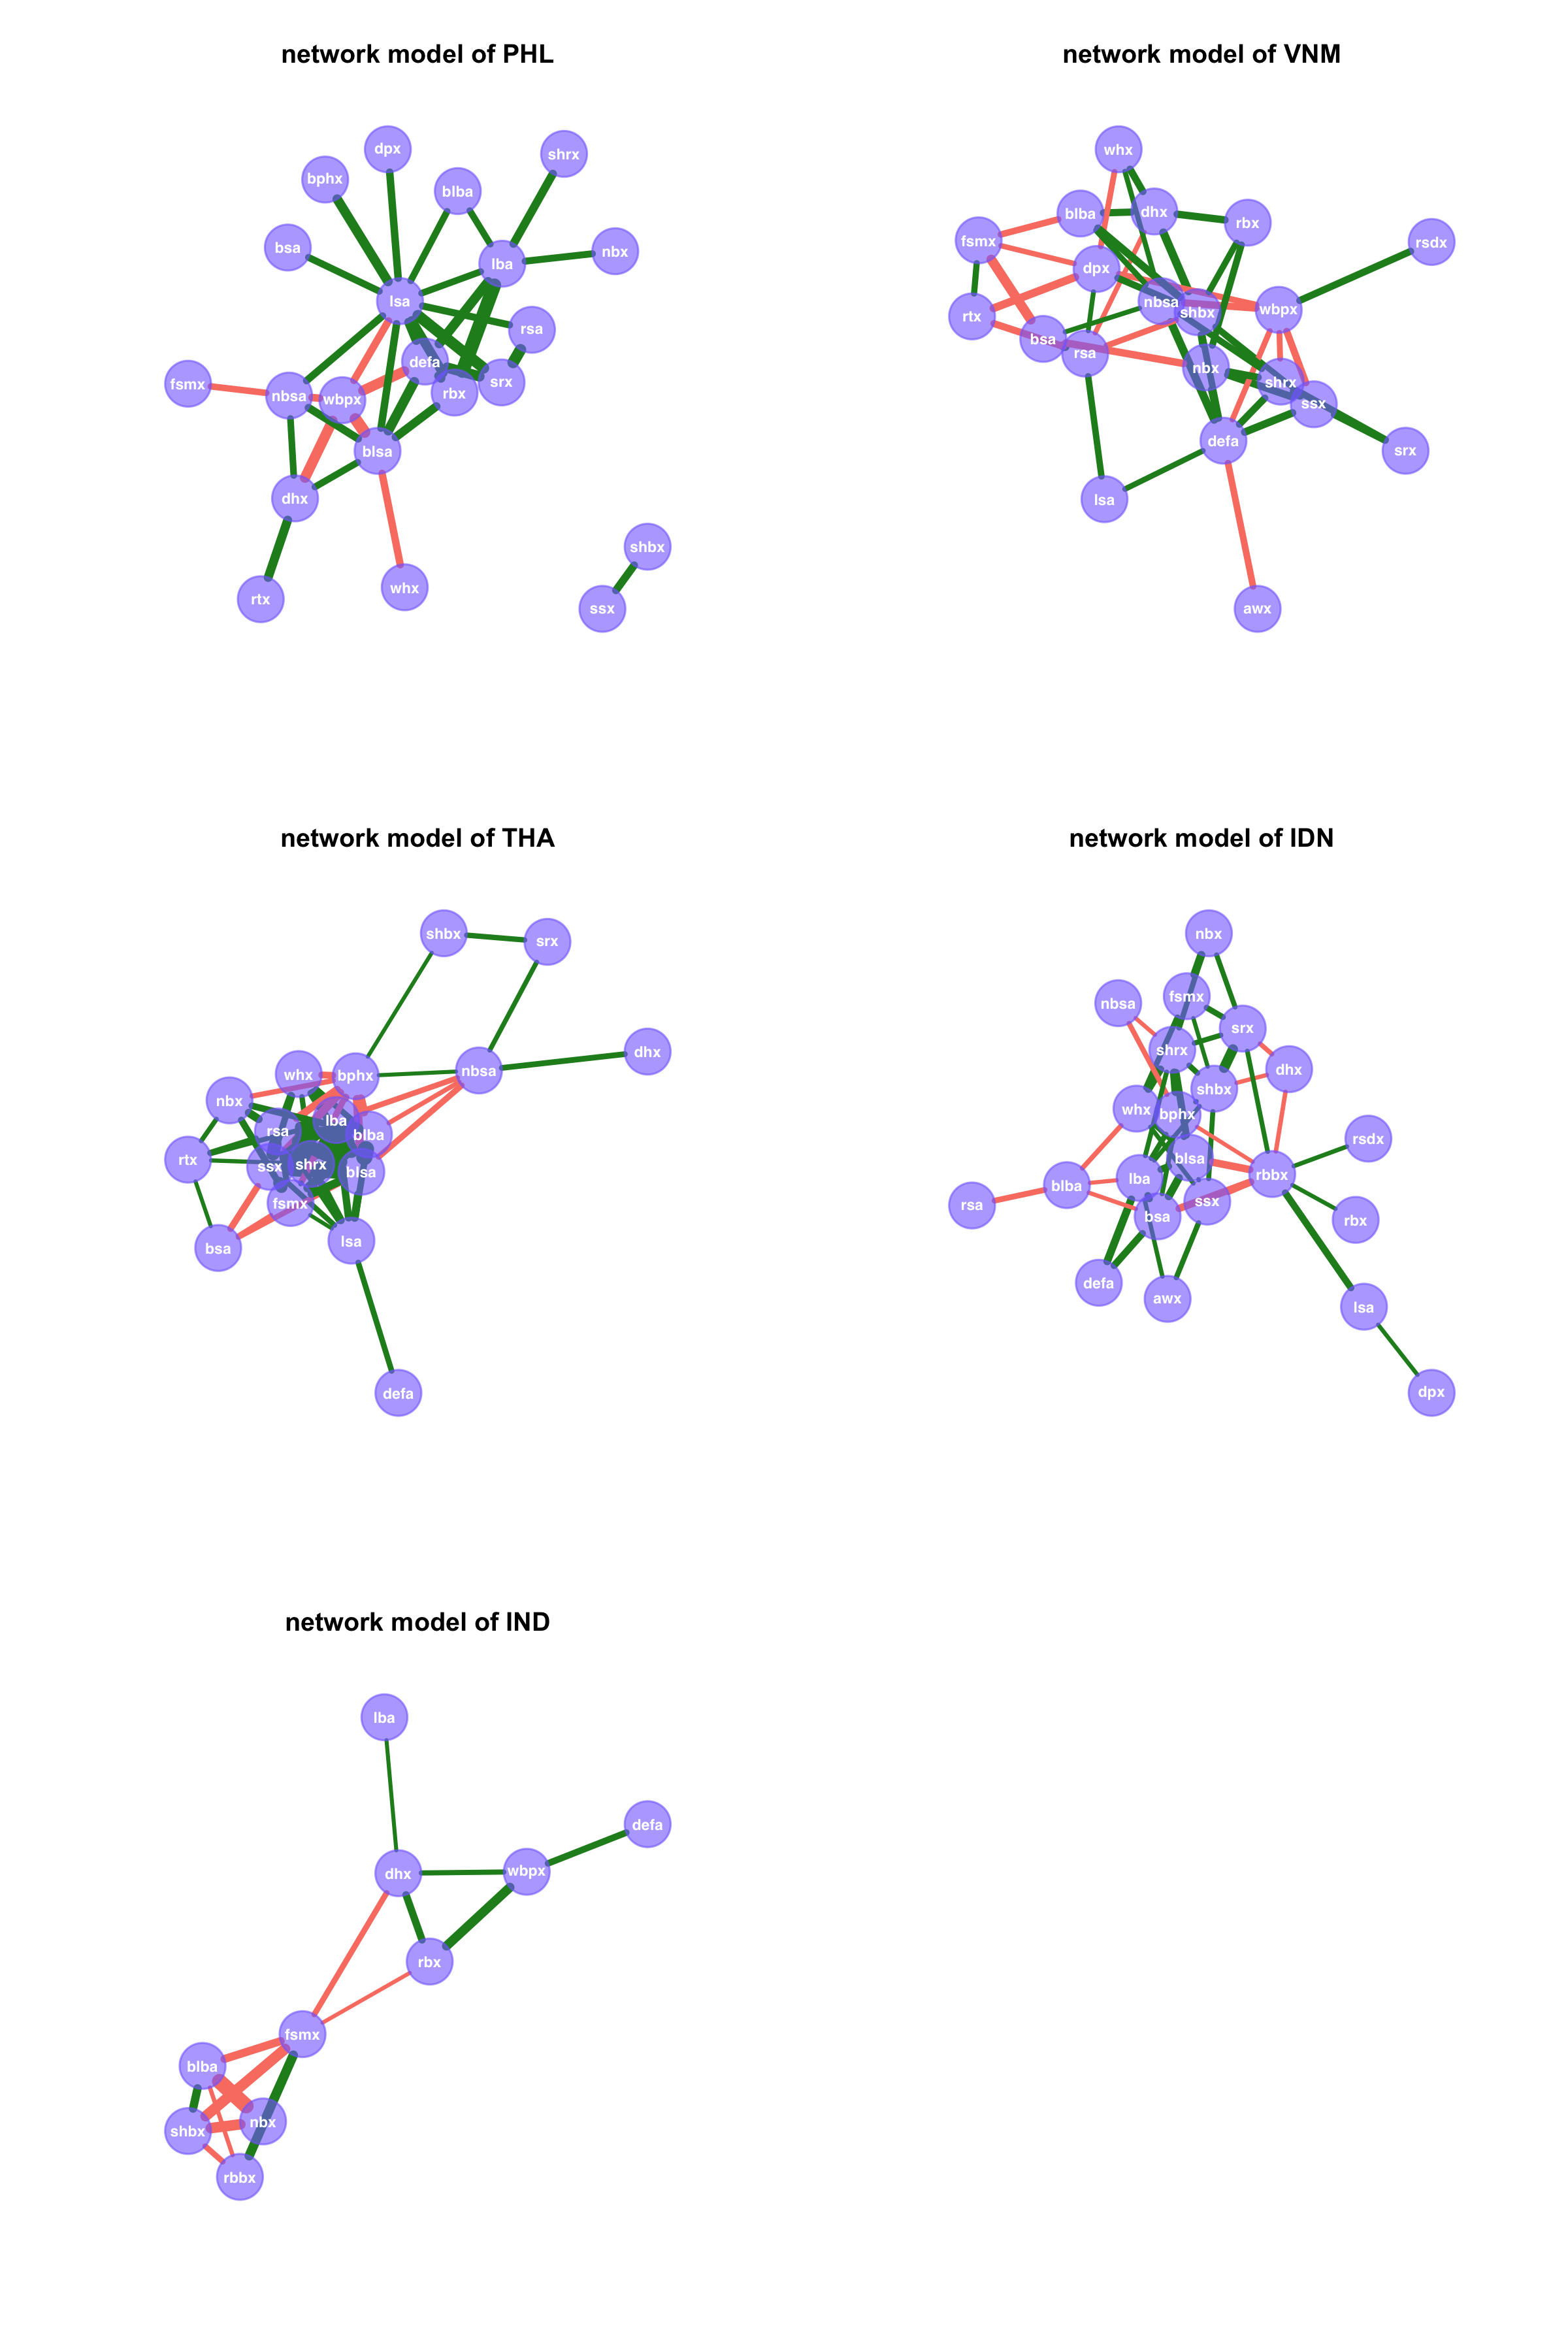
\includegraphics[width=15cm]{Netcountry}
\end{center}
 \textbf{\refstepcounter{figure}\label{Netcountry} Figure \arabic{figure}.}{ Enter the caption for your figure here.  Repeat as  necessary for each of your figures}
\end{figure}

\section*{Discussion}
\bibliographystyle{apalike}
\bibliography{ref}

\end{document}
